\documentclass{beamer}

\usepackage{amsmath, amssymb, hyperref, graphics, wasysym}
\usepackage{mathpazo}

\newcommand{\C}{\mathbb{C}}
\newcommand{\Z}{\mathbb{Z}}
\newcommand{\R}{\mathbb{R}}

\title{MAS439 Lecture 5 \\ Quotient Rings}

\date{October 11th}

\begin{document}

\begin{frame}
\titlepage
\end{frame}

\begin{frame}[plain,c]

\begin{center}

\Huge

\usebeamercolor[fg]{frametitle}
Announcements
\end{center}

\end{frame}

\begin{frame}{Homework 1: Whoops}

  \begin{block}{I didn't ask you to justify 1 and 3\dots}
    \dots but then marked them as if I did.
  \end{block}
  \begin{block}{I gave points back for those}
    Probably not reflected on homework you just corrected -- I made a copy of all homeworks, will add points back from those.
  \end{block}

  \begin{block}{In the future, you may lose points for not justifying things}
Lots of interesting philosophical questions about fairness, unspoken cultural assumptions, what's the point of pure maths: check the bulletin.

  \end{block}

  \end{frame}

\begin{frame}{Justify everything -- but briefly, humanely}
\begin{block}{Russell and Whitehead, Principia Mathematica}
  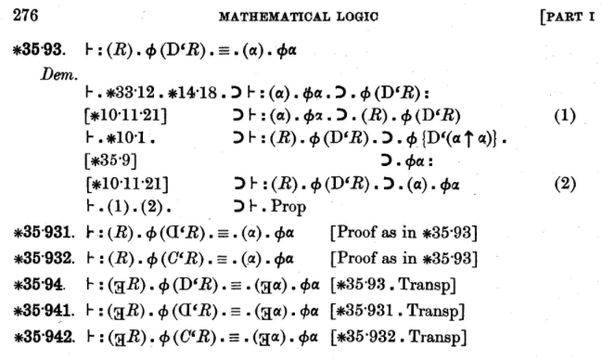
\includegraphics[width=\textwidth]{Principia.png}
\end{block}
\begin{block}{Thurston: Mathematics is for human understanding}
  \end{block}
\end{frame}

\begin{frame}{Homework 2: Whoops}
  \begin{block}{I forgot a minus sign. Two possible fixes:}
    \begin{itemize}
      \item Keep $\omega$ the same, but $\omega^2-\omega+1=0$
      \item Instead of $\omega$, use $$\rho=-1/2+i\sqrt{3}/2 $$
        Then $\rho^2+\rho+1=0$
    \end{itemize}
        Results in the same ring: $\{a+b\omega\}=\{c+d\rho\}$ because $\omega=\rho+1$.

\end{block}    
  \begin{block}{Sorry!}
    Proofs should go unchanged, won't lose marks because of this.
  \end{block}
\end{frame}


\begin{frame}{Pure Math Colloquia: Wednesdays at 2:00}
  \begin{block}{Theoretically, aimed to be understandable by all graduate students\dots}
    \dots but often fails that in practise.
  \end{block}
  Usually in J11.
  \begin{block}{Graduate student seminars/colloquia}
Not yet running/just starting.  A few fourth years attended last year; bug me next week or two if you're potentially interested.
  \end{block}

  \begin{block}{Next weeks colloquium should definitely be good, though}
  \end{block}  
\end{frame}


\begin{frame}{Pure mathematics in crisis}
  \begin{block}{Kevin Buzzard, Imperial College} Wednesday October 17, 2-3, Hicks Lecture Theatre C
  \end{block}

  \begin{block}{Abstract:}
I argue that pure mathematics is walking inexorably towards a cliff edge, and that anyone who believes that current pure mathematics is rigorous, or a science, needs to wake up and look at the facts, which there will be plenty of in this talk, and they are not pretty. Are our results reproducible? Does it matter? What *is* mathematics? Can computer scientists save us? Can *undergraduates* save us? I hope so. This talk is about pure mathematics but will be accessible to undergraduates, mathematicians both pure and applied/applicable and computer scientists. \end{block}
\end{frame}


\begin{frame}{Buzzard background reading I}
High mathematical drama
  \begin{block}{Mochizuki's ``proof'' of the ABC conjecture}
    \begin{itemize}
    \item ABC: roughly, let $a+b=c, a,b,c$ relatively prime, and $d$ be the product of distinct primes in $abc$.  Then $d$ is usually not much smaller than $c$.
    \item Put another way, if $a$ and $b$ have large powers of primes, then $c$ usually doesn't.
    \item Implies Fermat's last theorem $a^n+b^n\neq c^n$
    \item Shinichi Mochizuki has claimed a proof in 2012; 500 pages of very new mathematics, recently Peter Scholze has claimed a major gap.
      \end{itemize}

\end{block}
\end{frame}

\begin{frame}{Buzzard background reading II}
  More mathematical drama!
  \begin{block}{Hales's proof of the Kepler conjecture}
    \begin{itemize}
    \item Keper Conjecture: the densest way to pack three dimensional balls are how oranges are stacked in the grocers
    \item Hales and Ferguson gave a proof in 1998, involved lots of computer proofs
    \item Referees ran a seminar over several years to check it
    \item Published in 2005, but disclaimer that referees were only 98\% sure it was right
    \item ``Project Flyspeck'', a formal proof of the Kepler Conjecture, was completed in 2014
      \end{itemize}

  \end{block}

\end{frame}

\begin{frame}{The next few lectures: hard, so we're slowing down}
 
  \begin{block}{This week}
      \begin{itemize}
      \item[Thu:] Intro to quotient rings (Chapter 7)
      \item[Fri:] \begin{itemize}
      \item Examples of quotient rings (Chapter 7 + more)
      \item Thinking about quotient rings \\ \quad(Making things implicitly in notes explicit)
      \item Start category theory, universal property  \\ \quad(extra material + Chapter 8)
      \end{itemize}
      \end{itemize}
  \end{block}
  \begin{block}{Next week}
\begin{itemize}
  \item[Thu:] Isomorphism theorem (Chapter 8)
  \item[Fri:] I'll be gone.
    \begin{itemize}
    \item  Clean up?
      \item Maximal, Prime, radical ideals (Chapter 9)
      \end{itemize}
\end{itemize}        
        

\end{block}
\end{frame}
  


\begin{frame}[plain,c]

\begin{center}

\Huge

\usebeamercolor[fg]{frametitle}
Quotient Rings
\end{center}

\end{frame}



\begin{frame}{Goal:}
\begin{block}{Intuition: set everything in $I$ to be 0}
  Given a ring $R$ and an ideal $I\subset R$, construct a new ring $R/I$ and a homormophsim $p:R\to R/I$ so that
  \begin{itemize}
  \item $p$ is surjective
  \item $\ker(p)=I$
  \end{itemize}
  \end{block}
  \begin{block}{It's just like...}
    \begin{itemize}
    \item If $N\subset G$ a normal subgroup, we can make the quotient group $G/N$
      \item If $W\subset V$ a sub-vector space, we can make the quotient vector spave $V/W$.
    \end{itemize}
\end{block}
  \end{frame}

\begin{frame}{A first example: $\mathbb{Z}/n\mathbb{Z}$}
The map from $p:\mathbb{Z}\to\mathbb{Z}/n, p(k)=[k]_n$ is surjective, and has kernel $I=n\mathbb{Z}$.  

Thus when $I=(n)$, then $\mathbb{Z}/I=\mathbb{Z}/n\mathbb{Z}$.

\begin{block}{Something to keep in mind:}
We often \emph{think} ``$\mathbb{Z}/n\mathbb{Z}=\{0,1,2,\dots, n-1\}$.''

This isn't quite right, really:

$$\mathbb{Z}/n\mathbb{Z}=\{k+n\mathbb{Z} \}$$

We do this because awkward to think of ring elements as being themselves sets; and things in the second description have more than one name, i.e., $2+7\mathbb{Z}=-5+7\mathbb{Z}$.

\end{block}


\end{frame}


\begin{frame}{Review of quotient groups}
Recall that, given a normal subgroup $N \subset  G$, we have the quotient subgroup $G/N$.  The elements of $G/N$ are the \emph{cosets} of $N$ -- sets of the form $gN$.  Alternatively, elements of $G/N$ are equivalence classes, where $g\sim h$ if $gh^{-1}\in N$.

\begin{block}{Why did $N$ need to be normal?}
To make multiplication well defined.

\end{block}

\end{frame}





\begin{frame}{Definition of $R/I$ as a set}

As a set, the quotient ring $R/I$ is defined to be the set of equivalence classes under the relation $r\sim s$ if $r-s\in I$.

\begin{block}{Why?}
  Recall we want to build a map $p:R\to R/I$ with $\ker(p)=I$. We should have $r\sim s$ if $p(r)=p(s)$.  But:
  $$p(r)=p(s)\iff p(r-s)=0\iff r-s\in I$$
\end{block}
\begin{block}{Another perspective: cosets}
  The equivalence classes are exactly the sets of the form
  $$r+I=\{x\in R | x=r+i \text{ for some } i\in I\}$$
  \end{block}

\end{frame}


\begin{frame}{Operations on $R/I$}
We have defined what $R/I$ is as a set; we now need to turn $R/I$ into a ring.  We define addition and multiplication on $R/I$ by adding/multiplying representatives from the equivalence classes.  That is, 

$$[a]+[b]=[a+b]$$
$$[a]\cdot [b]=[a\cdot b]$$

\begin{block}{To show this makes $R/I$ into a ring we need to:}
\begin{itemize}
\item Check that these operations are well defined
\item Check that these operations satisfy the axioms of a ring
\end{itemize}
\end{block}

\end{frame}

\begin{frame}{Addition is well defined}
Suppose we chose $a^\prime\sim a$ and $b^\prime \sim b$.  For addition to be well defined we need:
$$[a^\prime+b^\prime]:=[a^\prime]+[b^\prime]=[a]+[b]=:[a+b]$$

\begin{itemize}
\item Since $a^\prime \sim a$, we have $a^\prime-a=i\in I$
\item Since $b^\prime \sim b$, we have $b^\prime-b=i\in I$ 
\item $(a^\prime+b^\prime)-(a+b)=(a^\prime-a)+(b^\prime-b)=i+j$
\item Since $I$ closed under addition, $i+j\in I$, so $(a^\prime+b^\prime)\sim (a+b)$
\end{itemize}

\end{frame}

\begin{frame}{Multiplication is well defined}
Suppose $$a^\prime-a=i\in I,\qquad b^\prime-b=j\in I$$  

We need to show that $$a^\prime\cdot b^\prime-a\cdot b\in I$$

Then:


$$a^\prime\cdot b^\prime-a\cdot b=(a+i)\cdot (b+j)-a\cdot b=a\cdot j+b\cdot i+i\cdot j$$

\begin{itemize}
\item Since $i, j\in I$ and $I$ an ideal, we have $a\cdot i, b\cdot j, i\cdot j\in I$. 
\item  Since $I$ is an ideal, their sum is also in $I$. 
\item  Hence $a^\prime\cdot b^\prime\sim a\cdot b$ and multiplication is well defined.
\end{itemize}

\end{frame}

\begin{frame}{$R/I$ satisfies the ring axioms}

These proofs are all just symbol pushing.  For instance, to show that the distributive law holds, we have:

\begin{align*}
([a]+^\prime[b])\cdot^\prime [c]& =[a+b]\cdot^\prime[c] \\
& =[(a+b)\cdot c] \\
&=[a\cdot c+b\cdot c] \\
&=[a\cdot c]+^\prime[b\cdot c]=[a]\cdot^\prime [c]+^\prime[b]\cdot^\prime [c]
\end{align*}

Here for clarity we use $+,\cdot$ for the operations in $R$ and $+^\prime, \cdot^\prime$ for the operations in $R/I$.
\end{frame}


\begin{frame}{In words}

That last proof was rather unenlightening. 
  
\begin{block}{ A paraphrase:}

The ring axioms are satisifed in $R/I$ because the operations $+, \cdot$ are defined in terms of lifting to representatives in $R$; and the axioms hold there.
\end{block}
\end{frame}


\begin{frame}[plain,c]

\begin{center}

\Huge

\usebeamercolor[fg]{frametitle}
Starting Examples
\end{center}

\end{frame}

\begin{frame}{Example: $\R[x]/(x^2)$}

First, we have to understand it as a set -- we want to give a \emph{unique} name to each element of $R/I$.  This is usually done by picking a representative from each coset in some systematic way.

$I$ consists of linear combinations of monomials of degree 2 or bigger.  So every equivalence class contains exactly one linear term $a+bx$.  We see that 

$$[a+bx]\cdot [c+dx]=[ac+adx+bcx+adx^2]=[ac+(ad+bc)x]$$


\end{frame}


\begin{frame}{Example: $\C\cong\R[x]/(x^2+1)$}

\begin{block}{The division algorithm gives unique representatives}

Any polynomial $p(x)$ can be written uniquely as

 $$p(x)=(x^2+1)q(x)+bx+a$$. 

This means that $[p(x)]=[bx+a]$, so every class can be represented by a linear polynomial; furthermore, this representation is unique.
\end{block}

It's clear $[a+bx]+[c+dx]=[a+c+(b+d)x]$.
\end{frame}

\begin{frame}{Example: $\mathbb{C}=\R[x]/(x^2+1)$}

\begin{block}{Multiplication of representatives}
$$[a+bx]\cdot [c+dx]=[ac+(ad+bc)x+bdx^2]$$

But this isn't linear;  we need to get rid of the $x^2$ term.  Note that $bdx^2=bd(x^2+1)-bd$, and so $[bdx^2]=[-bd]$.

Thus, we see
$$[a+bx]\cdot [c+dx]=[ac-bd+(ad+bc)x]$$
which, if we replace $x$ with $i$, is exactly the formula for multiplying complex numbers.
\end{block}


\end{frame}

\begin{frame}{Constructing $\mathbb{F}_4$}

We claim that $R=\mathbb{F}_2[x]/(x^2+x+1)$ is a field with 4 elements.  

Exactly as in the last two examples, the division algorithm gives every equivalence class has a unique linear representative $a+bx$; now $a,b\in\mathbb{F}_2$, so there are indeed four elements.

We check:
$$[x]\cdot [x+1]=[x^2+x]=[1]$$
So every nonzero element has an inverse, and so $R$ is a field.
\end{frame}




\end{document}
